\section{Introduction}\label{sec:intro}

Compiler design is a mature field with a wide range of well-known algorithms, with applications to code generation, static analysis, program transformation,
and more. The field also has seen the development of a number of mature
technology platforms which have enabled massive reuse across the compiler
community, including systems like the LLVM compiler
infrastructure~\cite{LLVM:CGO04}, the Java Virtual Machine (JVM)~\cite{Lindholm:1999:JVM:553607}, and many others.
A common characteristic of these popular systems is their ``one size fits all'' approach---a
\emph{single abstraction level} to interface with the system: the LLVM Intermediate Representation (IR) is
roughly ``C with vectors'', and JVM provides an ``object-oriented type
system with a garbage collector'' abstraction. This ``one size fits all''
approach is incredibly valuable---and in practice, the mapping to these
domains from ubiquitous source languages (C/\Cpp and Java respectively) is
straightforward.

At the same time, many problems are better modeled at a higher- or lower-level
abstraction, e.g.\ source-level analysis of \Cpp code is very difficult on LLVM
IR. We observe that many languages (including e.g.\ Swift, Rust, Julia, Fortran)
develop their own IR in order to solve domain-specific problems, like
language/library-specific optimizations, flow-sensitive type checking (e.g.\ for
linear types), and to improve the implementation of the lowering process.
Similarly, machine learning systems typically use ``ML graphs'' as a
domain-specific abstraction in the same way.

While the development of domain specific IRs is a well studied art, their
engineering and implementation cost remains high. The quality of the
infrastructure is not always a first priority (or easy to justify) for
implementers of these systems. 
Consequently, this can lead to lower quality compiler systems, including
user-visible problems like slow compile times, buggy implementations, suboptimal
diagnostic quality, poor debugging experience for optimized code, etc.

The \MLIR project aims to directly tackle these programming language design and
implementation challenges---by making it very cheap to define and introduce
new abstraction levels, and provide ``in the box'' infrastructure to solve
common compiler engineering problems. \MLIR does this by (1) standardizing the
Static Single Assignment (SSA)-based IR data structures,
(2) providing a declarative system for defining
\textit{IR dialects}, and (3) providing a wide range of common infrastructure
(including documentation, parsing and printing logic, location
tracking, multithreaded compilation support, pass management, etc).

This paper explores various design points of the \MLIR system, relates our
experience applying it to a number of different problems, and discusses
implications this work may have for language design and education.

\subsection{Contributions}

While most of the \MLIR system is built out of well known compiler algorithms,
the design points are sufficiently novel that it provides opportunities
for interesting research.  The contributions of this paper are:

\begin{itemize}
\item a description of a novel compiler infrastructure with important industrial and research applications;
\item new approaches to building scalable and modular compiler systems;
\item exploration of selected applications of \MLIR to diverse domains, illustrating the generality of the system;
\item shared experience developing systems that build on the \MLIR infrastructure.
\end{itemize}

\subsection{Where did \MLIR come from?}

Work on \MLIR began with a realization that modern machine learning frameworks
are composed of many different compilers, graph technologies, and runtime systems
(see~\figref{ml-compile})---which did not share a common infrastructure or design
point, and not all of which were following best practices in compiler design.
This manifested in multiple user-visible ways, including poor error messages,
failures in edge cases, unpredictable performance, and difficulty generalizing the
stack to support new hardware.

\begin{figure}[h]
  \centering
	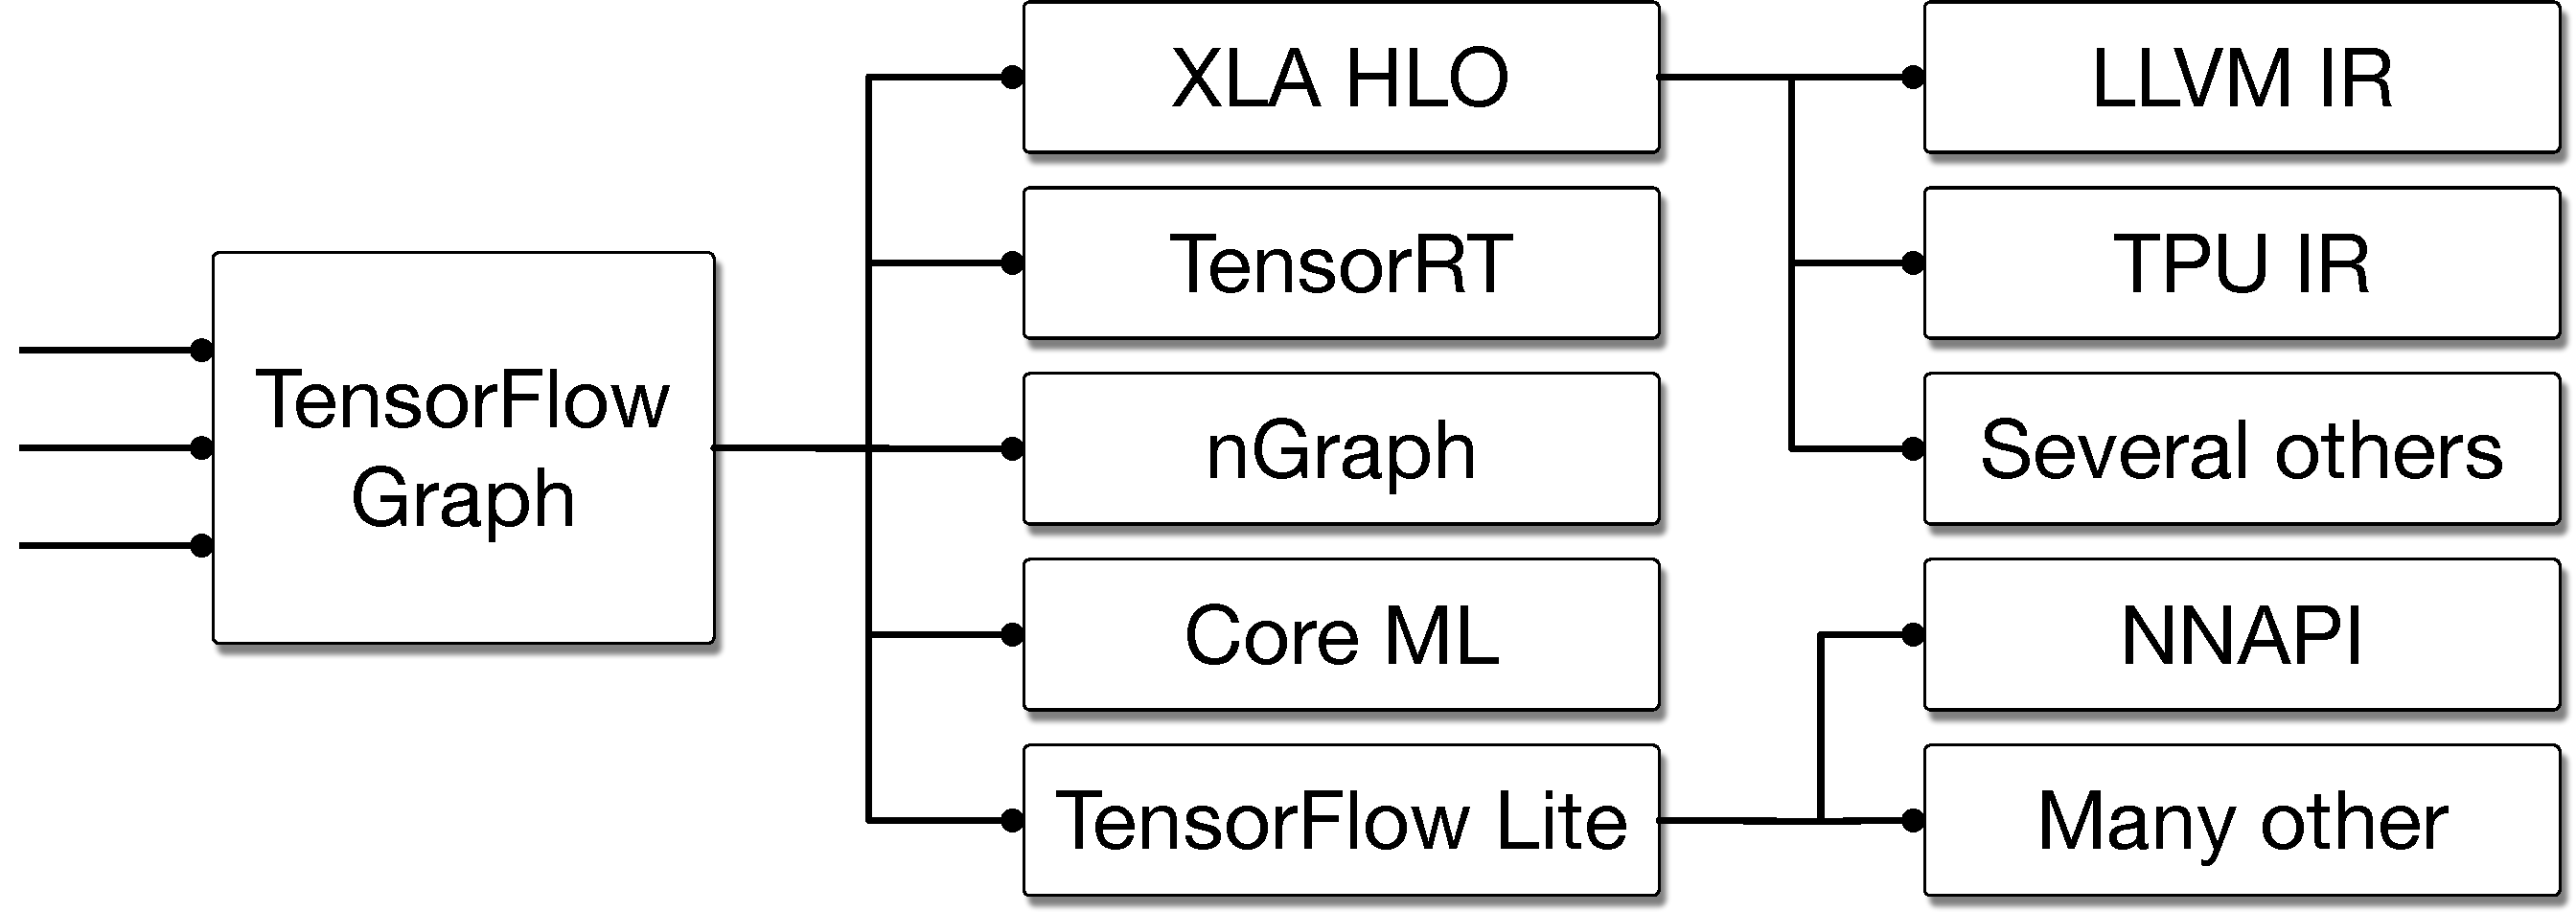
\includegraphics[width=0.7\textwidth]{img/tf_ecosystem_mono.pdf}
	\caption{TensorFlow model execution spanning different frameworks.}
  \label{fig:ml-compile}
\end{figure}

We soon realized that the compiler industry as a whole has a similar problem:
existing systems like LLVM are very successful at unifying and integrating work
across a range of different language implementations, but modern high level
languages often end up building their own high-level IR
and reinventing a lot of the same kinds of technology for higher levels of
abstraction (see~\figref{pl-midlevel}).  At the same time, the LLVM community
frequently struggled with questions about how to best represent parallel
constructs, how to share implementation of common front-end lowering infrastructure
(e.g.\ for C calling conventions, or cross-language features like OpenMP) with
no satisfactory solutions being available.

\begin{figure}[h]
  \centering
	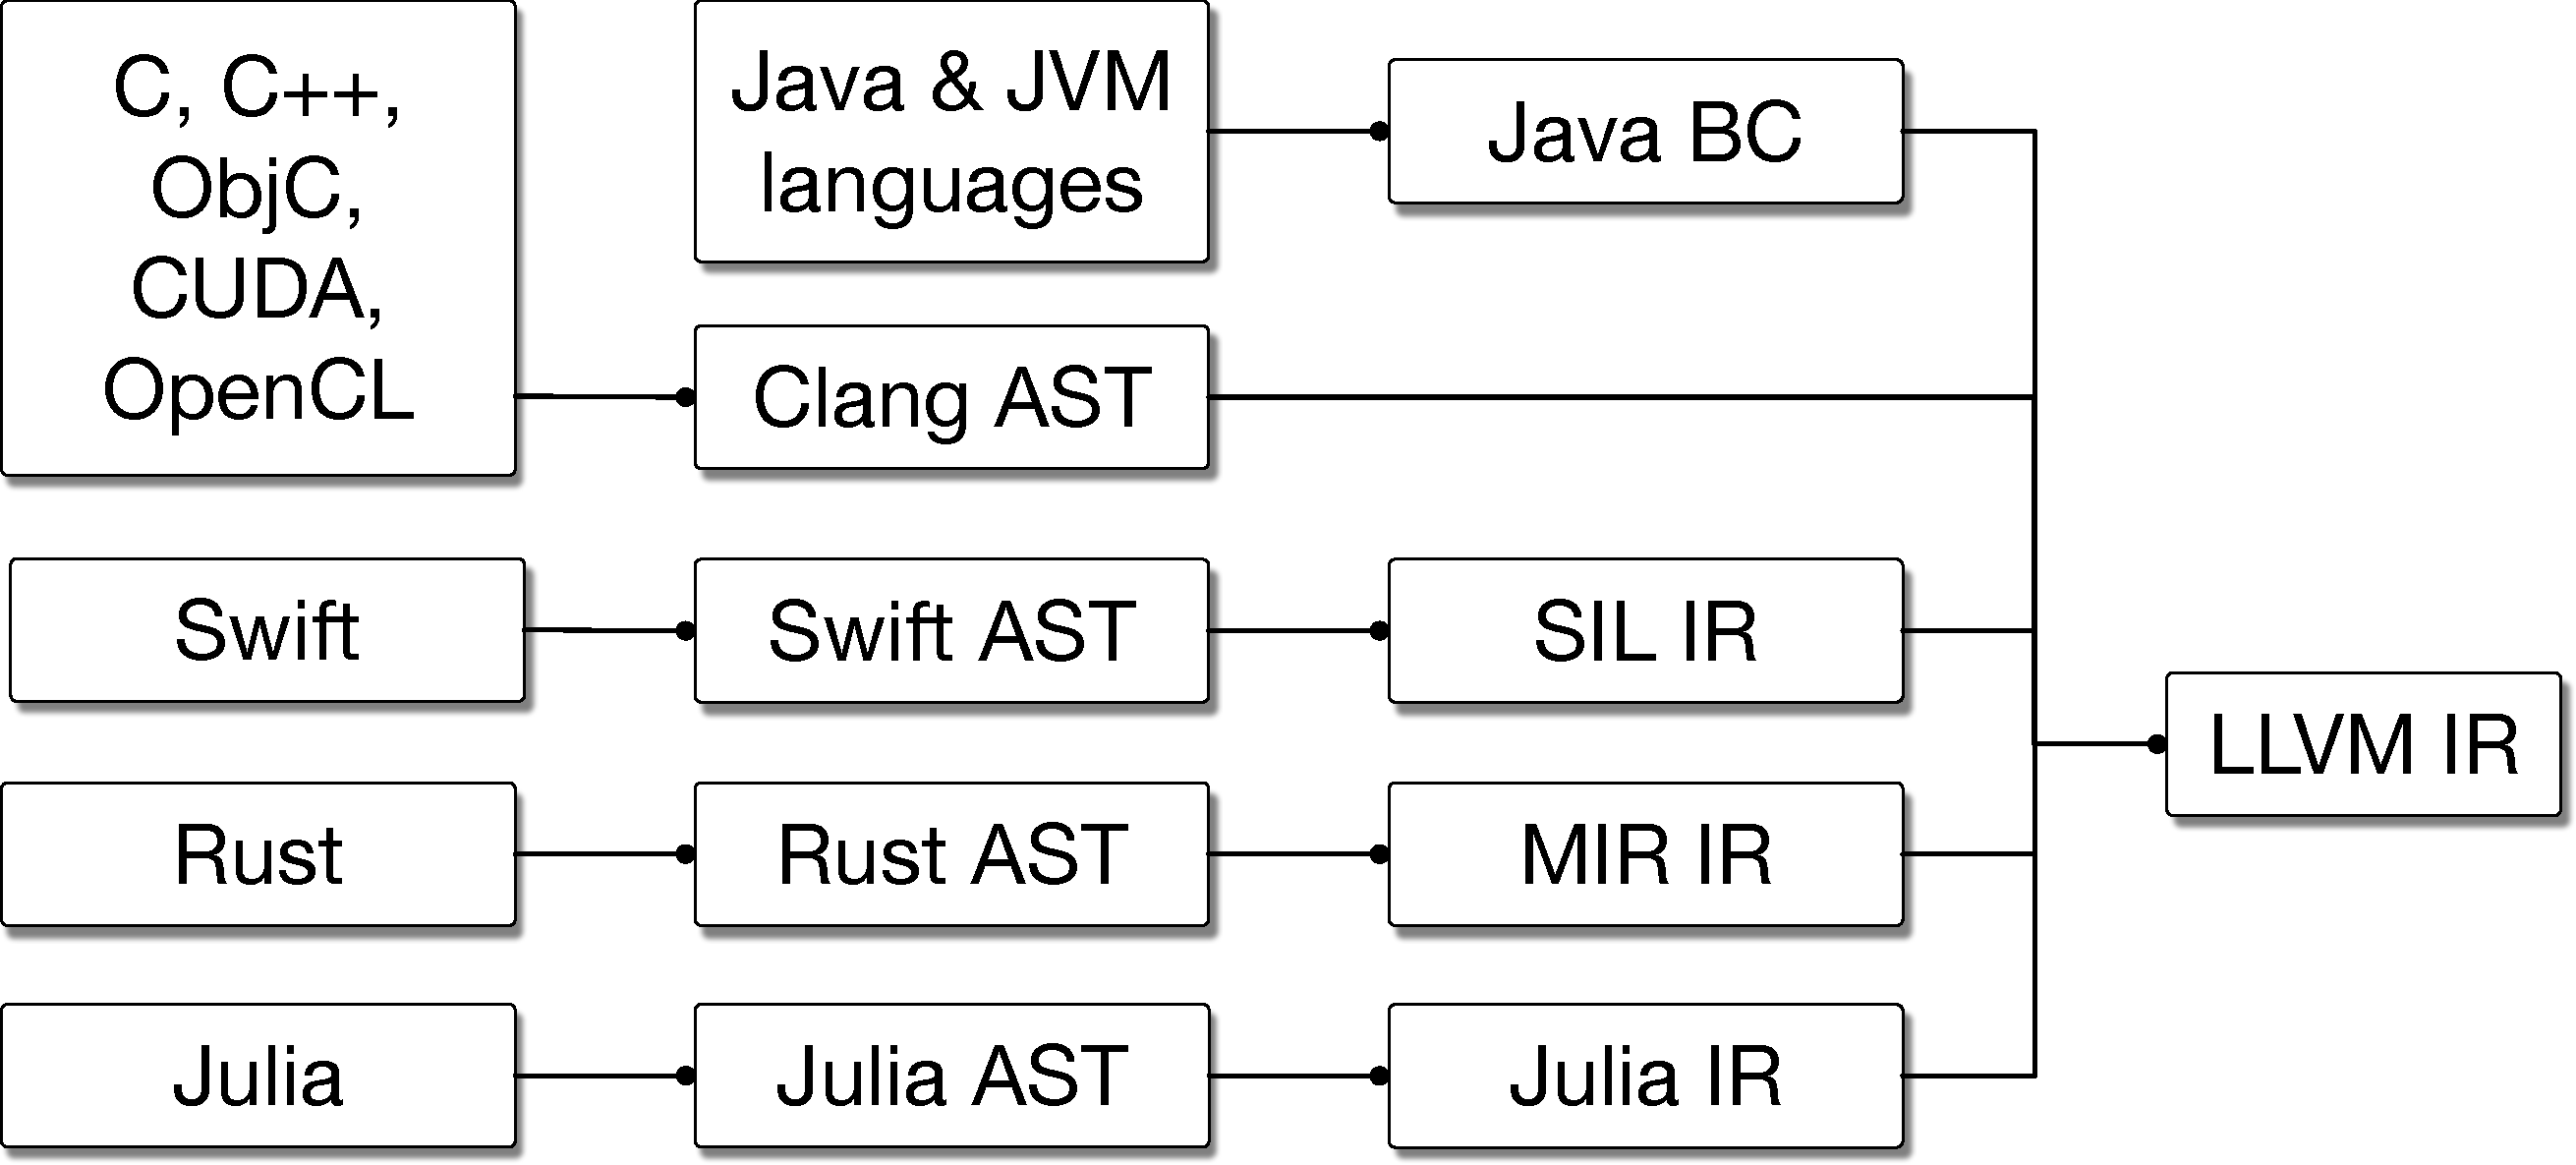
\includegraphics[width=0.7\textwidth]{img/domain_irs_mono.pdf}
	\caption{Compilation pipeline of different languages with multiple mid-level
    IRs for language-specific optimization with
    common backend for multiple hardware targets.}
   \label{fig:pl-midlevel}
\end{figure}

Faced with this challenge and perspective, we decided that we could not afford the
engineering effort to implement $N$ improved compiler instances, and we needed
to build a more general solution.  We reasoned that this would give us the ability
to invest in one set of high quality infrastructure which would benefit multiple
domains, would allow us to progressively upgrade existing systems in place,
would make it easier for us to tackle pressing problems like heterogeneous
compilation for specialized accelerators, and would provide interesting
research opportunities to define and explore.

Now that we have a significant amount of experience building and deploying
\MLIR-based systems, we are able to look back on the rationale and design of the infrastructure, and discuss why this direction was pursued.
